\section{Methodology}
From the many outlier detection methods introduced in the first section,
we carefully selected Pearson correlation coefficient, Singular
Spectrum Analysis and $k$-means for our study and tested them on ARM data. 

The various algorithms required differing levels of preprocessing. The
first level raw data was stored in minute resolution. It was normalized
for pairwise comparison algorithm. Some algorithms might not need
so much detail information to extract outliers. Thus we created a
second level data by averaging the minute data points into one
day point from the raw data. The second level data could save a lot
of running time and is easier for Plotly \cite{plotly} and
Matplotlib \cite{Hunter:2007} to visualize. The third level data
was specifically created for multivariate analysis by standardization
all the 5 variables into the same scale based on the second level
data. Below we will discuss each algorithm in detail. 

\subsection{Pearson correlation coefficient}
Co-located meteorological variables measure different aspect of the
atmospheric conditions at any location, and driven by atmospheric physics
are inherently correlated with each others. Any atmospheric phenomena at
the location would affect all variables in an expected
and correlated fashion.  Analysis of historical time
series data would provide us the baseline correlation structure and
patterns for the location. Any abrupt change or break in
correlation structure among meteorological behavior can be a sign of
sensor malfunction and should be identified as an outlier. In addition,
ARM SGP site comprise of multiple facilities making similar sets of
measurement and any abrupt change in correlation structure not observed
at other facilities will also indicate a potential outlier.

The Pearson correlation coefficient was first introduced by Karl
Pearson\cite{pearson1895note} and can be used to measure the linear
correlation between two variables. The Pearson correlation coefficient
is calculated from the covariance of two variables divided by the
multiplication of the standard deviation of those two variables. This
normalization results in a value between [-1, 1]. If the value is close
to -1, it means those two variables are highly negatively related. On
the other hand, if the value is close to 1, then the two variables are strongly positively related.
If the value is near 0, it means those two variables do not have linear
relation. 

\begin{figure*}[ht]
    \centering
    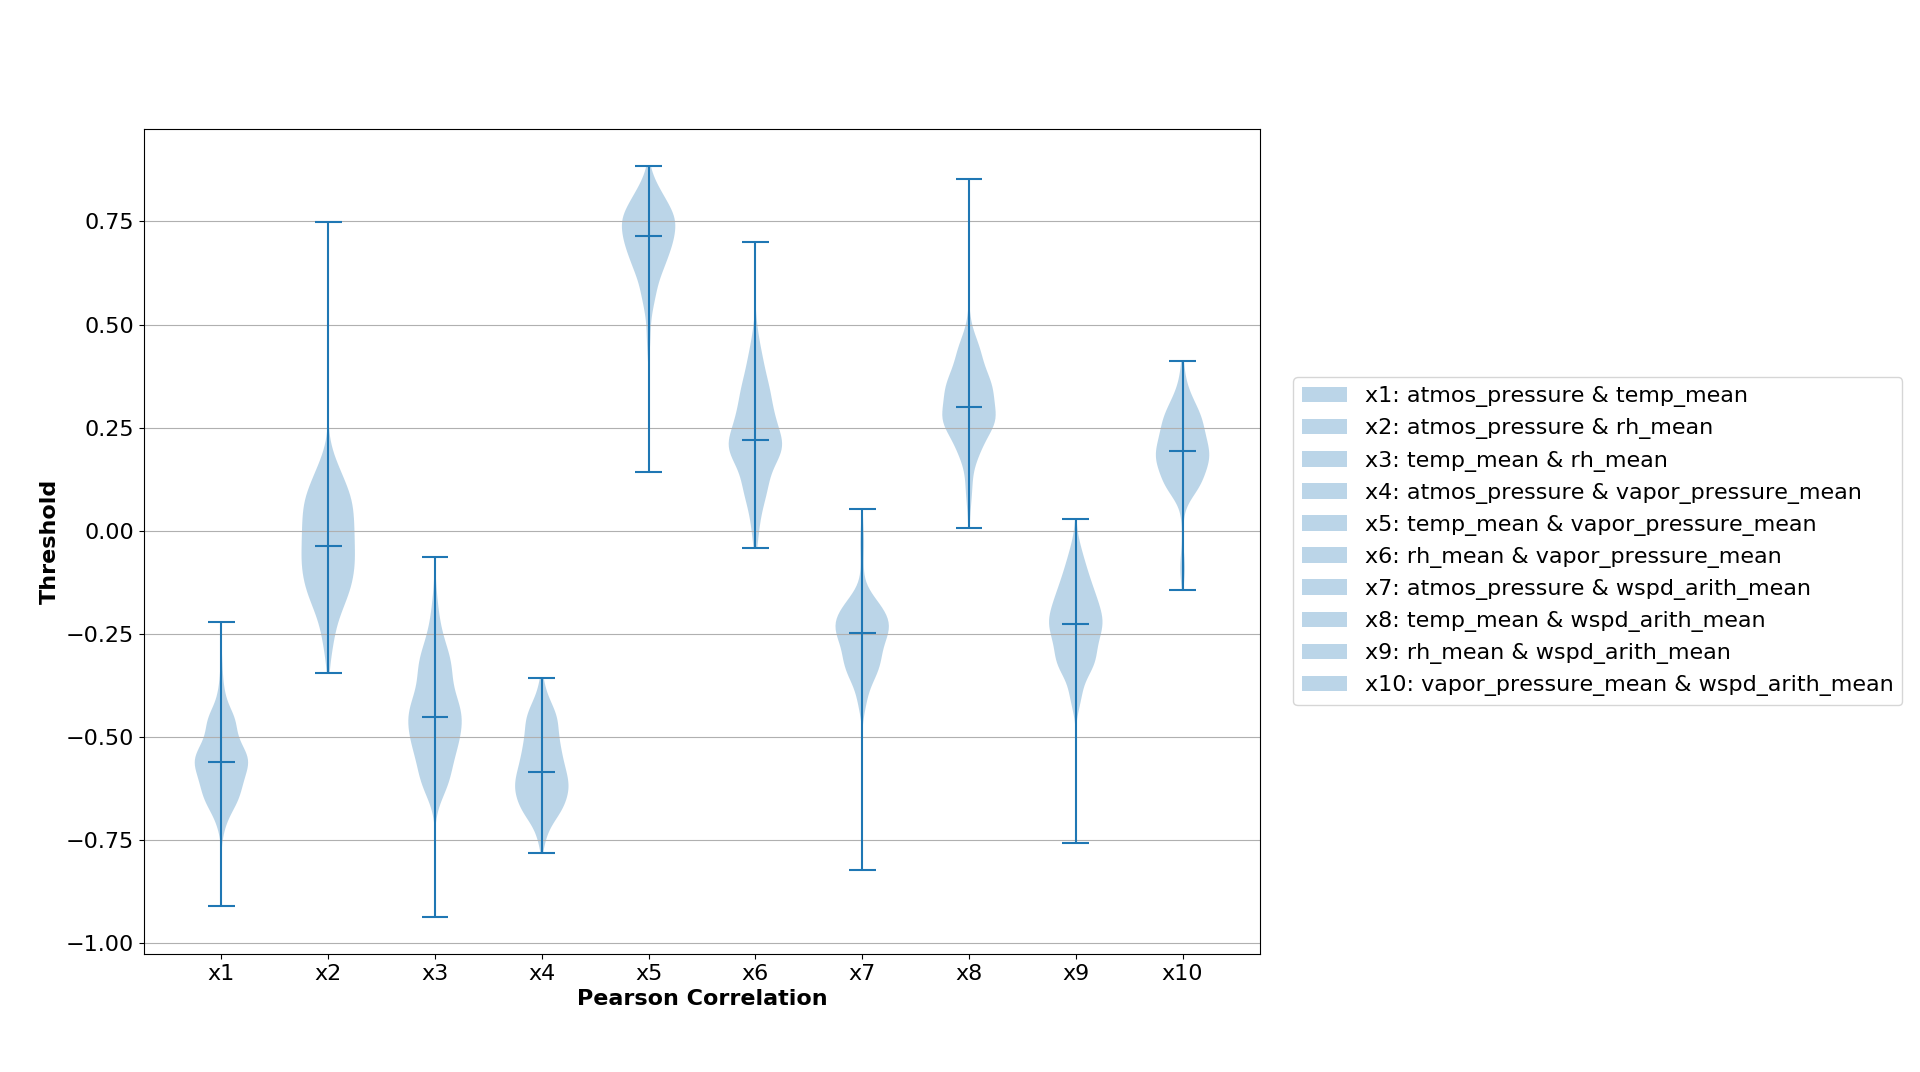
\includegraphics[width=\textwidth]{figures/Spring.png}
    \caption{Pearson Correlation patterns for ten meteorological variable pairs
		during spring season across all the years.}
    \label{fig:pc}
\end{figure*}

We performed a pairwise comparison of the five variables using Pearson
correlation using data from all 24 extended facilities. Atmospheric
dynamics are strongly driven by seasons and the correlation patterns
among meteorological variables can have season specific patterns. We
performed our analysis seasonally by separating the data among Winter, Spring,
Summer and Fall seasons. Figure~\ref{fig:pc} shows the distribution of
pairwise correlation for Spring season. All variables show strong
correlations which are normally distributed. The long tails of the
distribution are potentially due to outlier data points. 
For example, the Pearson correlation between
air temperature and vapor pressure is positively
correlated with correlation mean close to 0.75. And the Pearson
correlation between atmospheric pressure and air temperature is
negatively correlated with correlation mean close to -0.60. These highly
correlated Pearson correlation coefficients are stored as the expected
values between two variables. We then compare each Pearson correlation
of two variables from a specific season in a specific year from a
specific instrument individually. If this pairwise Pearson correlation
of two variables deviates far away from our expected historical
correlation, we treat it as an outlier. This method would allow to check
incoming datastream on near-real-time basis to identify outliers.

\subsection{Singular Spectrum Analysis}
Univariate time series analysis of meteorological variables can be
applied to identify any unexpected variability and extreme values
observed by the instruments. These anomalous observations can be
indicative of extreme atmospheric events at the site and are important
to identify. However, a range of natural inter-annual and intra-annual variability in
meteorological times series is also expected and it's important to not
erroneously flag them as outliers. We applied Singular Spectrum Analysis
for time series of analysis of meteorological observations to identify
extreme events.

Singular Spectrum Analysis (SSA) is a popular method for time series
data analysis \cite{golyandina2013singular,golyandina2014basic}. The
general idea is to use a subset of the decomposition of trajectory
matrix to approximate the original data. Many applications can be found
in \cite{golyandina2013singular}. For example, SSA can be applied to
monitor volcanic activity \cite{bozzo2010relationship}. It can also be
used to extract trend \cite{alexandrov2008method}. Different from the
classic SSA method, we defined our own version of SSA which is designed
to remove any number of modes of specified periodicity from the time
series. This is meant to remove known seasonalities from the data in 
order to isolate true anomalous values more accurately. 

\begin{figure*}[ht]
    \centering
    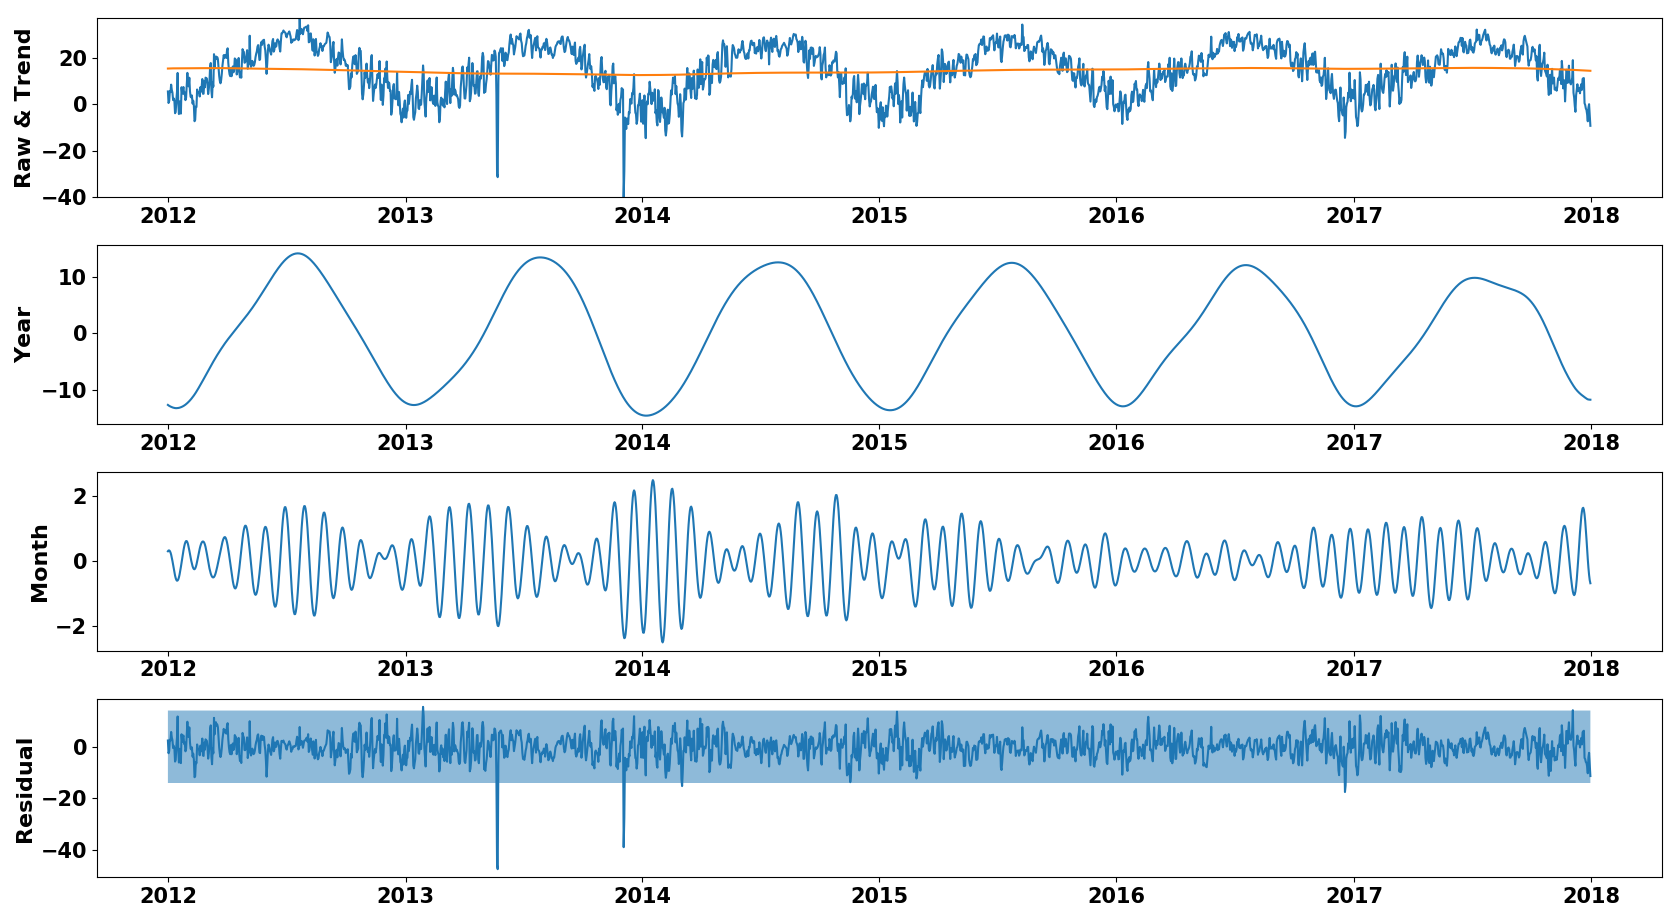
\includegraphics[width=\textwidth]{figures/E33.png}
    \caption{Decomposition of air temperature data from MET
		instrument at facility E33 using SSA method to isolate various
			frequencies.}
    \label{fig:ssa}
\end{figure*}

Assume we have an ARM time series data Y of length T
\begin{align*}
Y =(y_1,\ \ldots,\ y_T)
\end{align*}
where $T > 2$ and $y_i$ is not empty. Let $L\ (1 < L \leq T/2)$ be the window size and $K = T - L + 1$. In general, the algorithm contains two main parts: decomposition and reconstruction. The first step is to form the trajectory matrix \textbf{X} from vector Y by embedding subsets of Y. These subsets of Y $X_i$ are lagged vectors of length L.  
\begin{align*}
X_i = (y_i,\ \ldots,\ y_{L+i-1})^T \quad (1 \leq i \leq K) \\
\mathbf{X} = [X_1,\ \ldots,\ X_K] 
\end{align*}
Thus the trajectory matrix is
\begin{equation}
\mathbf{X} = (x_{ij})_{i,j=1}^{L,K}  = \left(\begin{IEEEeqnarraybox*}[][c]{,c/c/c/c/c,}
y_1 & y_2 & y_3 & \ldots & y_K\\
y_2 & y_3 & y_4 & \ldots & y_{K+1}\\
y_3 & y_4 & y_5 & \ldots & y_{K+2}\\
\vdots & \vdots & \vdots & \ddots & \vdots\\
y_L & y_{L+1} & y_{L+2} & \ldots & y_T
\end{IEEEeqnarraybox*}\right)\label{e:traj}
\end{equation}
where $x_{ij} = y_{i+j-1}$. We can see from equation 1 that matrix \textbf{X} has equal elements on anti-diagonals and therefore it is a Hankel matrix. Then we perform the singular value decomposition (SVD) on $\mathbf{S}=\mathbf{XX}^T$ where the eigenvalues of S are denoted by $\lambda_1, \ldots, \lambda_L$ in the decreasing order of magnitude $(\lambda_1 \geq \ldots \geq \lambda_L \geq 0)$ and the corresponding eigenvectors by $P_1, \ldots, P_L$. Let $d = rank\ \mathbf{X}$ and $V_i = \mathbf{X}^T P_i / \sqrt{\lambda_i} (i = 1, \ldots, d)$. Thus, the trajectory matrix X can then be written by its eigendecomposition,
\begin{equation}
\mathbf{X} = \mathbf{X_1} + \ldots + \mathbf{X_d}
\end{equation}
where $\mathbf{X_i} = \sqrt{\lambda_i} P_i V_i^T$.

Next we choose a subset of eigenpairs to form an approximation of the
trajectory matrix. It is at this point that our version of the algorithm
differs. Given that the time series we are studying has seasonality at
known frequencies, we use Fast Fourier transform (FFT) to find the
dominant frequency of each eigenvector \cite{cooley1965algorithm}. We
then approximate the trajectory matrix by including modes which match
the frequencies of the seasonality we wish to remove. For example, we
anticipate that the temperature data will have a annual and possibly
monthly cycle, as shown in Figure~\ref{fig:ssa}. SSA allows us to tease
out these contributions in additive fashion. In this example, the
signals from the year, month, and residual sum together to form the
original raw data. This residual is then the noise in the raw data with
the seasonality removed as doing so exposes large anomalies which are
possible outliers. 

Once the eigenpairs are chosen, we proceed with the classical definition
of the method. If $I$ represents a set of indices corresponding to the
eigenmodes to remove, we approximate the trajectory matrix
%
\begin{equation*}
    \mathbf{Xt} = \sum_{i\in I} \mathbf{X_i}
\end{equation*}
%
An approximation $Yt$ to the original signal $Y$ can be obtained from
$\mathbf{Xt}$ by inverting the process used to form the trajectory
matrix, Equation~\eqref{e:traj}. Each column of $\mathbf{Xt}$ represents
a shifted approximation to $Yt$, thus we average each shifted column.
Finally the deseasonalized residual is the difference between the
original signal and the reconstruction, $R=Y-Yt$.

We applied SSA for analysis of all five meteorological variables across
all facilities (Table~\ref{tab:datasets}) to identify outliers in all
meteorological observations.

Because SSA requires the time series data to be continuous, 
we corrected any missing values in the time series by replacing them
with long term seasonality. 
We set $L = 400$ and isolated the signals corresponding to year and
monthly frequency in the data.
Thus $Yt = Yt[0] + Yt[1] + Yt[2]$.
Figure~\ref{fig:ssa} show the result of SSA analysis for
air temperature variable at facility E33. The first row of
Figure~\ref{fig:ssa} show the raw daily time series ($Yt$) of
air temperature, which show no significant trend (orange line
$Yt[0]$) at the site during period 2012 to 2017.
The second and third rows show the annual ($Yt[1]$) and monthly
($Yt[2]$) frequencies of the temperature time series respectively. 
Temperature time series data show strong annual and monthly frequencies
at the sites which expected and reflective of long term weather patterns
experienced at the SGP site. 
The last row show the time series of residual after removing the tends,
and annual and monthly frequencies from the data. While some of the
residuals may be reflective if natural variability, the
anomalous positive or negative temperature residuals can be identified
as outliers in the data. Multiple methods are available to set a threshold 
for extreme values in the residuals as outliers. We used the three sigma 
rule to extract outliers \cite{pukelsheim1994three}. For example, the two
peak points in Figure~\ref{fig:ssa} are larger than three sigmas, 
thus are outliers.

\subsection{K-means}

Southern plains, where SGP site is located, are known to experience frequent extreme
storms occurring most frequently during spring and early summer seasons.
Identifying these extreme events is of interest for scientific users of
the data to study and/or isolate these phenomena. However,
meteorological variables during such events won't be captured by Pearson
Correlation as they may still follow know correlation structure at seasonal scales
or by SSA method since any individual variable may not
show large deviation. Multivariate approach like $k$-means clustering
have been widely used to identify weather and climate regimes
\cite{Hoffman_EI_20050803,Hargrove_EnvironManage_20040401}. We used
$k$-means clustering algorithm to delineate the weather regimes at SGP
site. While extreme storms and weather events that often occur at sub-daily
timescales may still fall within identified known weather regimes at the
site, they often are out of norm extremes within the regime and of
interest to us.

K-means is a partitioning clustering algorithm \cite{macqueen1967some,
hartigan1979algorithm}. It starts with user specified $k$ centroids, 
and assigns the points to the nearest centroid. Then it
computes new $k$ centroids and assigns all data points to these
centroids again. This process is repeated until convergence criteria is
met. 

% K-means algorithm
\begin{algorithm}[ht]
\DontPrintSemicolon
\SetAlgoLined
%\KwResult{Dominant frequency of each eigenvector}
\SetKwInOut{Input}{Input}
\SetKwInOut{Output}{Output}
\Input{ARM time series data}
\Output{Outliers}
\BlankLine

outliers $\leftarrow \varnothing$\;
df $\leftarrow$ ARM time series data\;
data $\leftarrow$ df[`atmos\_pressure',`temp\_mean',\
`rh\_mean',`vapor\_pressure\_mean',`wspd\_arith\_mean']\;
number\_of\_clusters $\leftarrow$ 4\;
clusters $\leftarrow$ K-means(data, number\_of\_clusters)\;
distances $\leftarrow$ Distance between each point and its centroid\;
mean $\leftarrow$ arithmetic mean of distances\;
sigma $\leftarrow$ standard deviation of distances\;
threshold $\leftarrow$ mean + 3 * sigma\;
\For{i in range(size of distances)}{
    \If{distances[i] $>$ threshold}{
        outliers $\leftarrow$ outliers $\cup$ {distances[i]}
    }
}
\Return outliers
\caption{K-means Outlier Detection}\label{alg:kmeans}
\end{algorithm}

We applied $k$-means clustering to ARM meteorological data set to
defined weather regimes at SGP site. We then calculated the distance of
each point within a cluster to its corresponding cluster centroid.
Vector of distances within each cluster were used to identify points
that are on fringes of the regime they belong to and considered
outliers. All five meteorological variables were used in this analysis.
Algorithm~\ref{alg:kmeans} describes the workflow.

\begin{figure*}[ht]
    \centering
    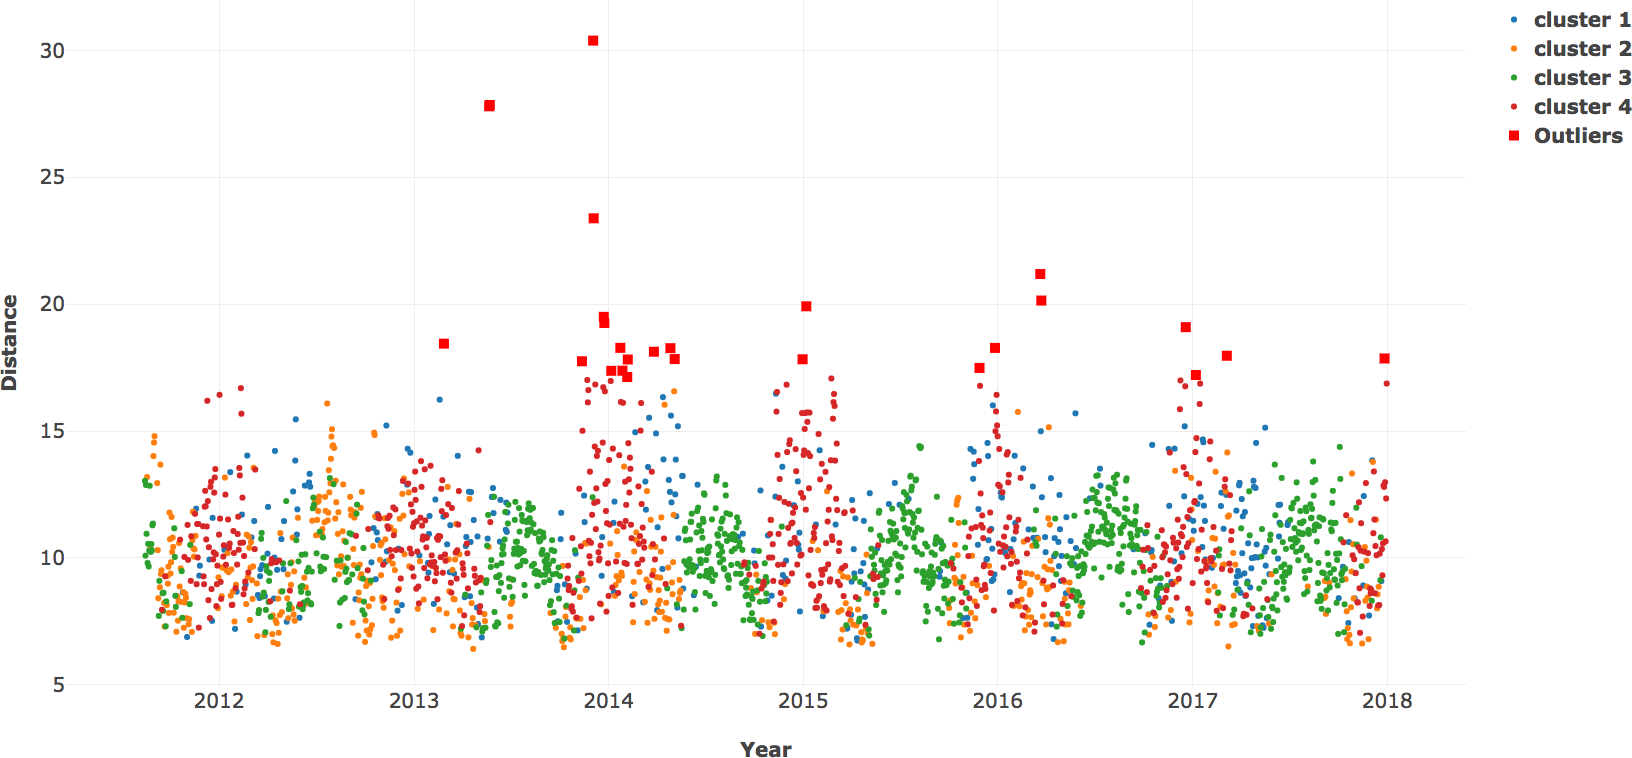
\includegraphics[width=\textwidth]{figures/kmeans.png}
    \caption{Outliers detected using $k$-means method at facility E33.
		$X$-axis represent the daily meteorological time series, colored
		by cluster (weather regime) they belong to, while
		$Y$-axis show the distance of the data point from the centroid
		of its cluster (weather regime).}
    \label{fig:kmeans}
\end{figure*}
% cluster 1: oct - june spring 
% cluster 2: sept - mar fall/winter 
% cluster 3: may - oct  summer
% cluster 4: jan - may fall

Given known seasonal patterns at the site we set $k$ to four to
determine weather regimes for four seasons. Figure~\ref{fig:kmeans}
shows the four regimes at facility E33 that representing spring (cluster
1), winter (cluster 2), summer (cluster 3) and fall (cluster 4).
Data points within each weather regime (or cluster) that are at
significant distance from their clusters (identified by red squares in
Figure~\ref{fig:kmeans}) were identified as outlier (and may correspond
to extreme weather events).

\subsection{Evaluation of outlier detection}
ARM data quality assurance program maintains a database of outliers that
has been been identified, inspected and documented for all historical
data. However, recorded data quality
issues are added manually for historical data when an issue is
identified or reported and are known to be incomplete \cite{mccord2016arm}. 
A description of the outlier event is included in these DQR which often
are temporary change in operating conditions such as power failures, frozen 
and snow covered sensors, instrument degradation, or contamination. 
Most often extreme weather events are not captured and reported by the
current system before. Each DQR entry also contains a specific time range affected, 
list of data projects, and specific measurements. And these entries 
are usually submitted by either the Data Quality Office \cite{peppler2016arm} 
or the instrument mentor \cite{cress2016deploying}. 
The Data Quality Reports (DQR) are stored and available as PostgreSQL
database (\url{http://dq.arm.gov}). 
We evaluated outliers
identified by methods developed in this study against the DQRs in the
database through database queries and calculated \textit{Precision} and \textit{Recall}
metrics \cite{perry1955machine}. We treated outliers in DQR database as True Positives. 
The equation \ref{eq3} and \ref{eq4} show the calculation of \textit{Precision} and \textit{Recall}.

\begin{table*}[ht]
\begin{equation}\label{eq3}
\mathbf{Precision} = \frac{\mathbf{True\ Positives}\ (Outliers\ detected\ in\ DQR\ database)}{\mathbf{True\ Positives + False\ Positives}\ (Outliers\ detected\ not\ in\ DQR\ database)}
\end{equation}

\begin{equation}\label{eq4}
\mathbf{Recall} = \frac{\mathbf{True\ Positives}\ (Outliers\ detected\ in\ DQR\ database)}{\mathbf{True\ Positives + False\ Negatives}\ (Undetected\ records\ in\ DQR\ database)}
\end{equation}
\end{table*}

